\section{FuzzBench Experimental Results}

\subsection{RQ1: Basic Effectiveness}

\begin{figure}
  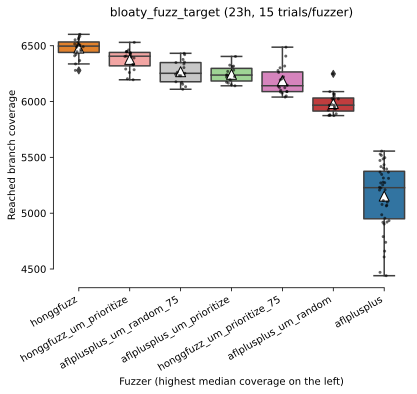
\includegraphics[width=0.75\columnwidth]{bloaty_fuzz_target_boxplot.pdf}
  \caption{AFLplusplus with and without (random) mutant fuzzing: final branch coverage}
  \label{fig:bloatybox}
  
\end{figure}

\begin{figure}
  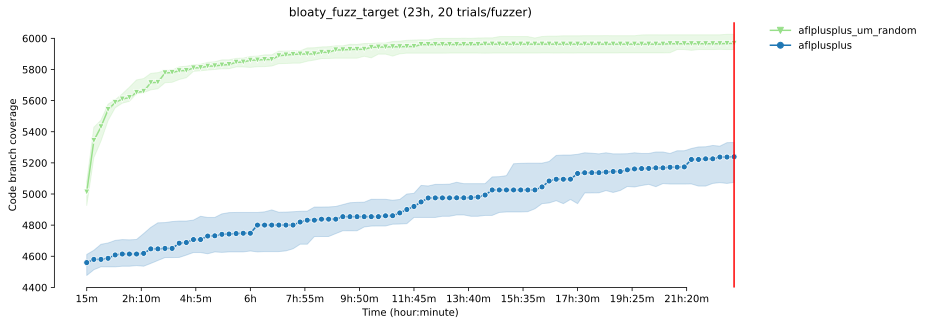
\includegraphics[width=0.75\columnwidth]{bloaty_fuzz_target_coverage_growth.pdf}
  \caption{AFLplusplus with and without (random) mutant fuzzing: branch coverage growth}
  \label{fig:bloatygrowth}  
  \end{figure}

  Figures \ref{fig:bloatybox} and \ref{fig:bloatygrowth} show that in some cases the impact of analyzing mutants can be a large improvement in code coverage.  In all of our FuzzBench results, {\tt um\_random} indicates fuzzing including mutants, without mutant prioritization; similarly, {\tt fuzzername\_um\_prioritize} would indicate fuzzing with baseline fuzzer {\tt fuzzername} and prioritized mutants.  We indicate deviations from our default 0.50 mutant-fuzzing budget by appending the fraction of the overall fuzzing budget spent on mutants, e.g., {\tt honggfuzz\_um\_prioritize\_75} would indicate fuzzing using Honggfuzz on prioritized mutants, where only the last 25\% of the fuzzing budget was spent fuzzing the original program.

Bloaty (\url{https://github.com/google/bloaty}) is not a toy program; like all FuzzBench benchmarks, it is a real-world program, in this case with nearly 4,000 GitHub stars, and over 7,700 lines of code.  Baseline AFLplusplus weak performance shows that it is not an easy target to fuzz effectively.  Such dramatic improvements, with an effect size of hundreds of branches, with a Mann-Whitney U-test $p$-value of less than 0.001, and a 1.0 probability that mutant-based fuzzing outperforms the base fuzzer, were rare.  However, the overall results support the utility of our approach, using AFLplusplus (\url{https://github.com/AFLplusplus/AFLplusplus}) and Honggfuzz (\url{https://github.com/google/honggfuzz}) as our baseline fuzzers:

  \begin{itemize}
  \item Using the first of FuzzBench's standard evaluation measures, ``based on the average of per-benchmarks scores, where the score represents the percentage of the highest reached median code-coverage on a given benchmark (higher value is better)'', the best performing fuzzer in our experiments was AFLplusplus using prioritized mutants, with a normalized score of 97.91.  The next best fuzzer, AFLplusplus without mutants, had a score of 97.64.  Honggfuzz with prioritized (97.45) or randomly chosen (97.0) mutants also performed better than baseline Honggfuzz (96.97) by this measure.
    \item Using the other standard FuzzBench evaluation measure, ``average rank of fuzzers, after we rank them on each benchmark according to their median reached code-covereges (lower value is better)'', AFLplusplus with prioritized mutants again scored best (average rank of 3.11), and all AFLplusplus mutant variations performed better than baseline AFLplusplus.  Honggfuzz however, scored better than all mutant variants of Honggfuzz.
    \end{itemize}

    \begin{table}
      \begin{tabular}{l|r|r}
        Fuzzer & Average Normalized Branch Coverage \\
        \hline
        \hline
aflplusplus\_um\_prioritize & 97.91 \\
aflplusplus & 97.64 \\
aflplusplus\_um\_random\_75 & 97.60 \\
honggfuzz\_um\_prioritize & 97.45 \\ 
honggfuzz\_um\_random & 97.00 \\
honggfuzz & 96.97 \\
aflplusplus\_um\_random & 96.16 \\
honggfuzz\_um\_prioritize\_75 & 96.15 \\
honggfuzz\_um\_random\_75 & 95.29 \\
      \end{tabular}
      \caption{Ranking by Average Normalized Branch Coverage}
      \label{tab:rankings1}
    \end{table}

    \begin{table}
      \begin{tabular}{l|r|r}
        Fuzzer & Average Fuzzer Rank \\
        \hline
        \hline
aflplusplus\_um\_prioritize & 3.11 \\
aflplusplus\_um\_random\_75 & 3.27 \\
aflplusplus\_um\_random & 3.32 \\
aflplusplus & 3.52 \\
honggfuzz & 3.82 \\
honggfuzz\_um\_prioritize & 4.13 \\
honggfuzz\_um\_prioritize\_75 & 4.90 \\
honggfuzz\_um\_random\_75 & 5.00 \\
honggfuzz\_um\_random & 5.18 \\
      \end{tabular}
      \caption{Ranking by Average Fuzzer Rank}
      \label{tab:rankings2}
    \end{table}
    
Tables \ref{tab:rankings1} and \ref{tab:rankings2} show full results for these core FuzzBench multi-benchmark evaluations, for the nine configurations we were able to run.  The absence of non-cumulative variants, as well as of bug-based evaluations, is explained below (see Section \ref{sec:fuzzexp}).


\begin{table}
  {\scriptsize
    \begin{tabular}{l||r|r|r|r||r|r|r|r|r}
      Benchmark & \multicolumn{4}{|c||}{AFLplusplus} & \multicolumn{5}{|c}{Honggfuzz} \\
      \hline
     & & prioritize & random & random\_75 & & prioritize & random & prioritize\_75 & random\_75 \\
        \hline
        \hline
bloaty\_fuzz\_target & 79.20 & 94.73 & 90.39 & 94.79 & 98.40 & 97.03 & 95.58 & 93.02 & 92.94 \\
curl\_curl\_fuzzer\_http & N/A & N/A & N/A & N/A & 99.01 & N/A & N/A & N/A & N/A \\
freetype2-2017 & 90.33 & 91.58 & N/A & 91.33 & 95.19 & 95.65 & N/A & 96.06 & 96.02 \\
harfbuzz-1.3.2 & 95.01 & 94.43 & N/A & 95.28 & 94.07 & 94.63 & 94.51 & 94.26 & N/A \\
jsoncpp\_jsoncpp\_fuzzer & 99.04 & N/A & N/A & N/A & 99.42 & 99.81 & N/A & 99.81 & N/A \\
lcms-2017-03-21 & 91.94 & 91.91 & 92.03 & N/A & 66.81 & 88.32 & N/A & 71.31 & N/A \\
libjpeg-turbo-07-2017 & 97.71 & 97.99 & 98.04 & 97.75 & N/A & 96.08 & 92.67 & 96.13 & 96.18 \\
libpcap\_fuzz\_both & 89.47 & N/A & 71.78 & N/A & 86.96 & 87.31 & N/A & 85.28 & 85.43 \\
libpng-1.2.56 & 93.02 & N/A & N/A & 93.10 & 95.05 & 97.17 & 95.36 & 95.05 & 97.97 \\
libxml2-v2.9.2 & 86.09 & N/A & N/A & N/A & 91.23 & N/A & 90.98 & 90.72 & 90.51 \\
libxslt\_xpath & 98.84 & N/A & N/A & N/A & 97.78 & N/A & N/A & N/A & N/A \\
mbedtls\_fuzz\_dtlsclient & 78.28 & 78.62 & N/A & 78.71 & 77.18 & 76.69 & 77.00 & 77.01 & N/A \\
openssl\_x509 & 99.97 & 99.89 & 99.89 & 99.85 & 99.54 & 99.48 & N/A & 99.43 & N/A \\
openthread-2019-12-23 & 92.93 & N/A & N/A & N/A & 92.12 & 79.22 & 91.09 & 78.73 & 77.38 \\
php\_php-fuzz-parser & 98.76 & 99.10 & 99.07 & 99.18 & 99.04 & 98.89 & 98.78 & 98.56 & 98.58 \\
proj4-2017-08-14 & 86.82 & 89.33 & N/A & 89.50 & 96.11 & 96.43 & N/A & 95.34 & N/A \\
re2-2014-12-09 & 99.32 & 98.60 & 98.56 & 98.58 & 98.52 & 98.58 & N/A & 98.54 & N/A \\
sqlite3\_ossfuzz & 94.03 & 83.39 & 81.42 & 84.56 & 81.49 & 81.12 & 80.73 & 81.02 & 79.07 \\
systemd\_fuzz-link-parser & 100.00 & 100.00 & 100.00 & 100.00 & N/A & 99.15 & 99.15 & 99.15 & N/A \\
vorbis-2017-12-11 & 98.67 & 98.67 & 98.82 & 98.67 & 97.65 & 97.53 & 97.49 & 97.61 & N/A \\
woff2-2016-05-06 & 97.62 & 97.78 & 97.78 & 97.66 & 96.18 & 96.39 & N/A & 96.51 & N/A \\
zlib\_zlib\_uncompress\_fuzzer & 97.98 & N/A & N/A & 94.90 & N/A & 97.98 & N/A & 98.51 & 97.45 \\
\hline
Median & 95.01 & 96.26 & {\bf 98.04} & 95.28 & 96.11 & 96.43 & 94.51 & 95.70 & 94.48 \\
Mean & 93.57 & 94.00 & 93.43 & {\bf 94.26} & 92.72 & 93.55 & 92.12 & 92.10 & 91.15 \\
      \end{tabular}
      }
      \caption{Full Median Relative Branch Coverage Results for FuzzBench Benchmarks}
      \label{tab:fullfuzzbench}
    \end{table}

    Finally, Table \ref{tab:fullfuzzbench} shows complete results for all benchmarks and fuzzers.  {\bf N/A} indicates that a particular run failed, usually due to build issues; note that this sometimes happened, due to the stress on the build assumptions discussed below, even for baseline fuzzers.  The median and mean fuzzer statistics here are computed without the normalization used in the standard rankings shown above, but are still indicative of overall fuzzer performance, assuming no bias in missing results, and are of course valid for use in comparing pairs of fuzzers on a single benchmark.  Again, methods using mutants scored highest for both median and mean branch coverage.  To see full results, including statistical significance (most differences were significant at the $p$ < 0.05 level), please see the complete FuzzBench generated report merging all of our experiments (\url{https://github.com/agroce/fuzzing22report/blob/master/fuzzbench_report_10_17/report}).  The original experiment runs are available at the FuzzBench site (\url{https://fuzzbench.com/reports/experimental/2022-10-13-um-final-1/index.html}, \url{https://fuzzbench.com/reports/experimental/2022-10-13-um-final-2/index.html}, \url{https://fuzzbench.com/reports/experimental/2022-10-13-um-final-4/index.html}, and \url{https://fuzzbench.com/reports/experimental/2022-10-13-um-final-5/index.html}).

    While our results are limited, we note that mutants seemed to have better impact on AFLplusplus than on Honggfuzz.  Even so, out of  the 16 benchmarks where we have results for both base Honggfuzz and and Honggfuzz over prioritized mutants, the prioritized approach performs better in terms of median branch coverage for 9 benchmarks.  Moreover, the impact was sometimes large:  for the lcms-2017-03-21 benchmark, for example, baseline Hongfuzz only covered a median of 66.81\% of the best achieved branch coverage; using prioritized mutants improved this to a median of 88.32\% of best branch coverage, with a $p$-value of < 0.05.

\subsubsection{Individual Benchmark Fuzzing Impacts}
    
Restricting our attention to comparisons of AFLplusplus with AFLplusplus over randomly chosen mutants for half the fuzzing budget, we can observe that the effect of fuzzing mutants can be dramatic, and can vary considerably.  We focus on randomly chosen mutants despite the overall superior performance of prioritized mutants in order to show that even with random selection of mutants, the variance for fuzzing can in many cases be no greater than for fuzzing without mutants.  Full results for this comparison can be examined in the FuzzBench report repository: \url{https://fuzzbench.com/reports/experimental/2022-10-13-um-final-1/index.html}.

\begin{figure}
  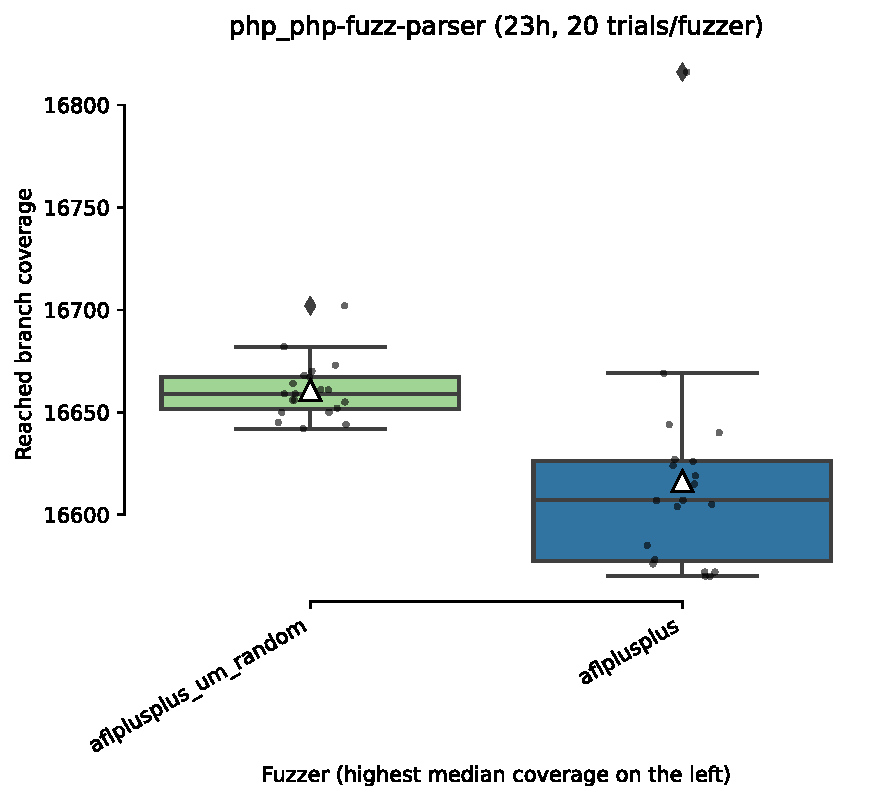
\includegraphics[width=0.75\columnwidth]{php_php-fuzz-parser_boxplot.pdf}
  \caption{AFLplusplus with and without (random) mutant fuzzing: final branch coverage}
  \label{fig:phpbox}
  
\end{figure}

\begin{figure}
  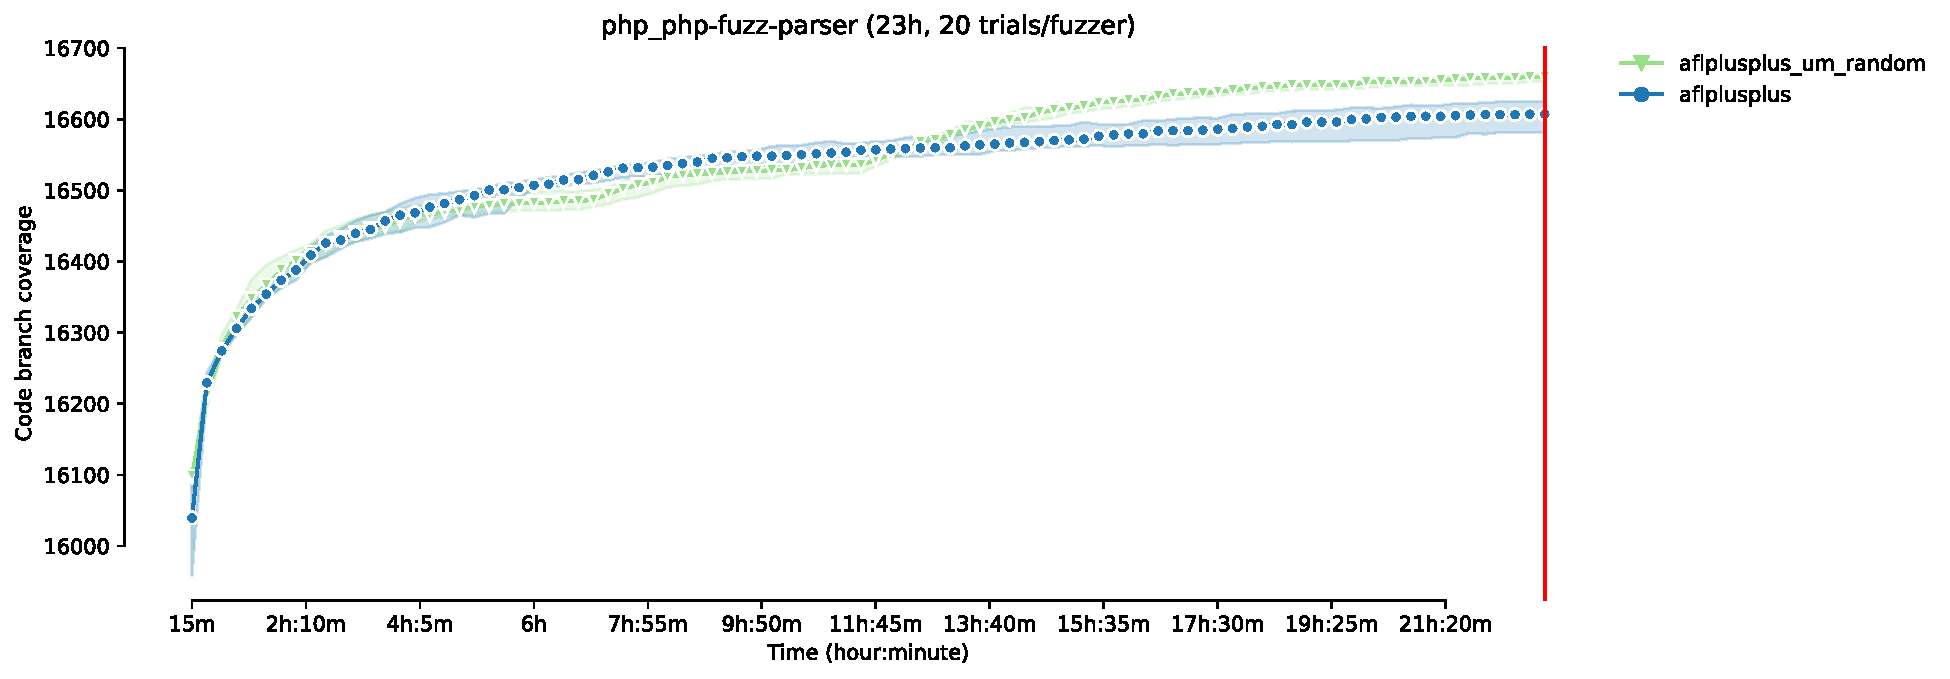
\includegraphics[width=0.75\columnwidth]{php_php-fuzz-parser_coverage_growth.pdf}
  \caption{AFLplusplus with and without (random) mutant fuzzing: branch coverage growth}
  \label{fig:phpgrowth}  
\end{figure}

Figures \ref{fig:phpbox} and \ref{fig:phpgrowth} show that the impact of mutant fuzzing is not always, as with the bloaty benchmark, evident during the mutant-fuzzing phase.  Here, the (consistent) advantage over AFLplusplus only appears after fuzzing has swiched to the original target program.  Presumably, seeds generated by some mutants ``pay off'' during the final run of original-target fuzzing.  Again we note that many mutants are likely essentially equivalent in their impact on fuzzing, since the confidence intervals on branch coverage are tight despite the use of randomly selected, likely non-overlapping, mutants in these runs and the bloaty runs.

\begin{figure}
  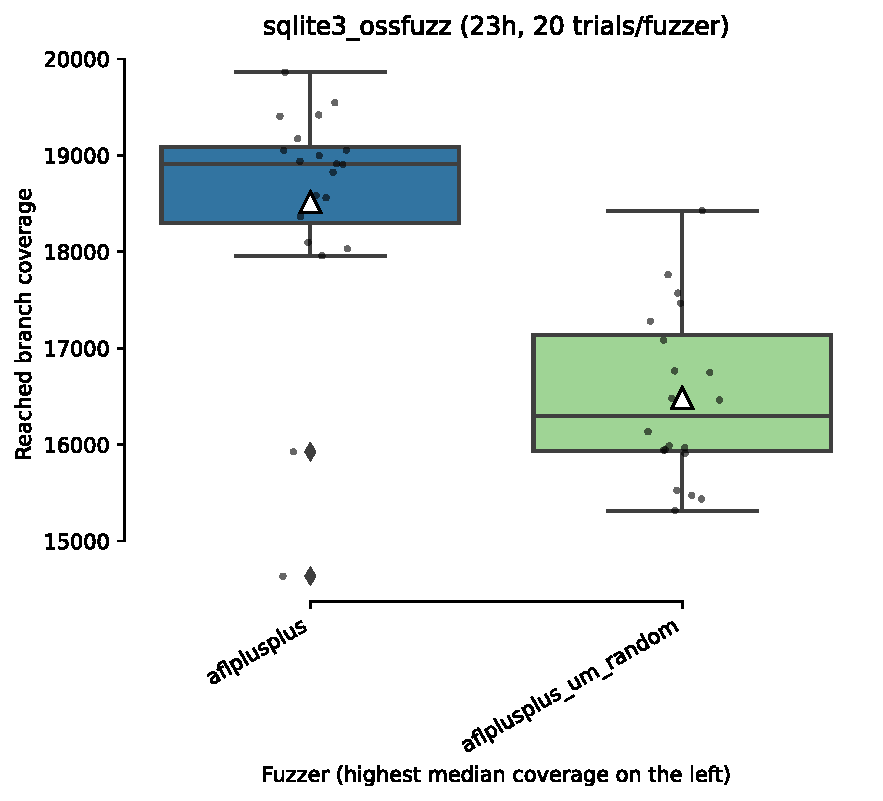
\includegraphics[width=0.75\columnwidth]{sqlite3_ossfuzz_boxplot.pdf}
  \caption{AFLplusplus with and without (random) mutant fuzzing: final branch coverage}
  \label{fig:sqlitebox}
  
\end{figure}

\begin{figure}
  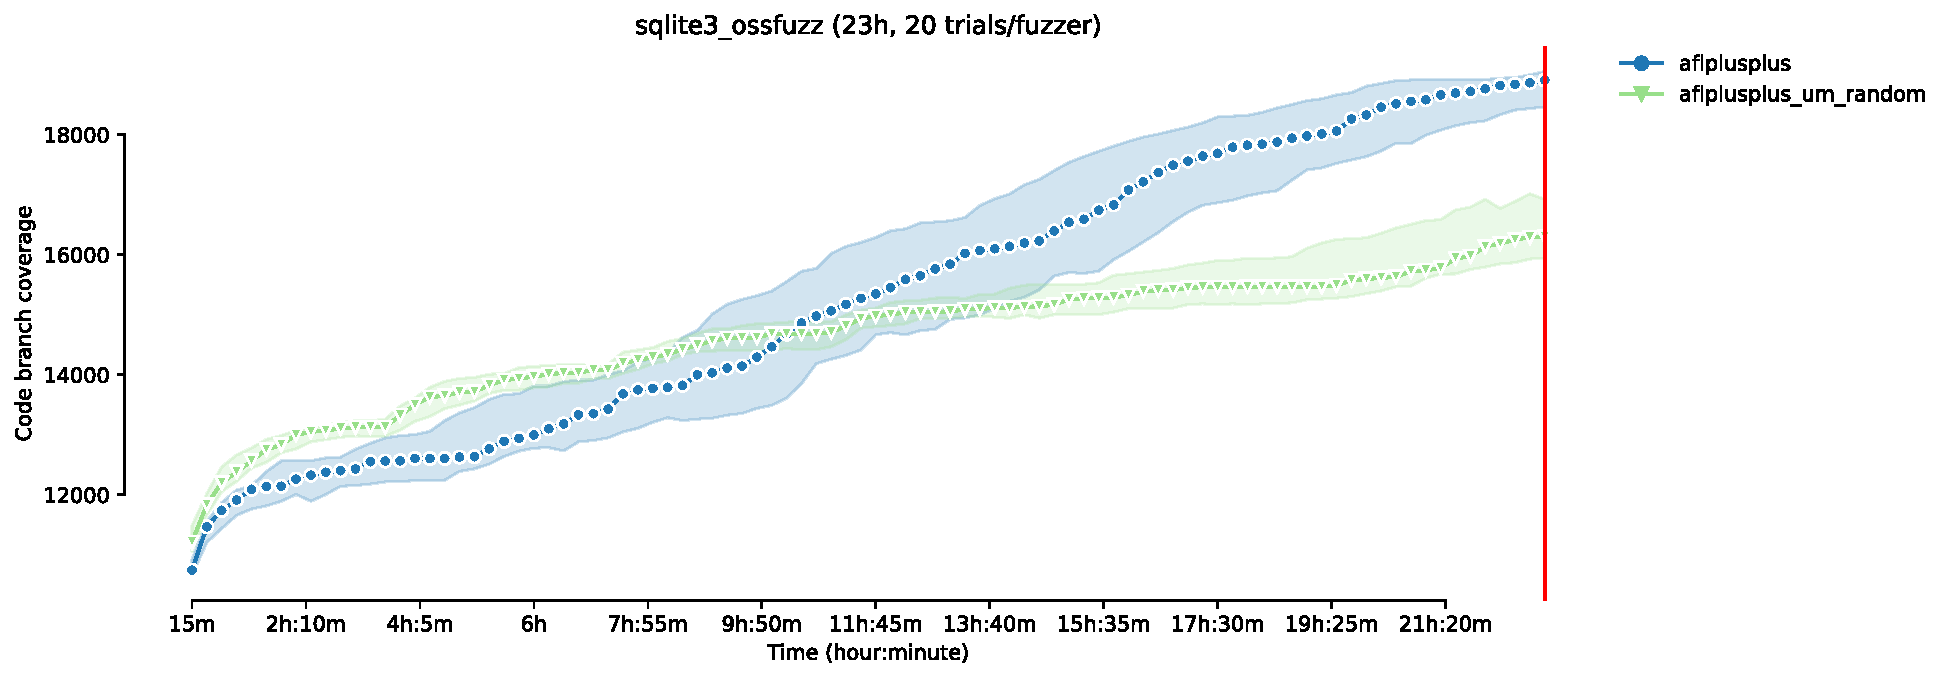
\includegraphics[width=0.75\columnwidth]{sqlite3_ossfuzz_coverage_growth.pdf}
  \caption{AFLplusplus with and without (random) mutant fuzzing: branch coverage growth}
  \label{fig:sqlitegrowth}  
\end{figure}

Finally, it is not always the case that mutants having a strong impact on fuzzing pays off in the long run.  Figures \ref{fig:sqlitebox} and \ref{fig:sqlitegrowth} show that fuzzing mutants can provide a statistically significant advantage over a baseline fuzzer early in the run, but eventually ends up performing significantly worse over a longer period.  We are not sure what causes such results: one possibility is that many mutants are harmful, and the useful mutants that cause the early advantage help with overcoming fuzzing barriers that also can be defeated simply by using a good fuzzer for a longer period.

 \subsection{RQ2: Effects of Mutant Prioritization}

In all cases, the prioritized variants of the approach scored better than using randomly chosen mutants.  We would need more fuzzers to be sure that this effect persists across all fuzzers, but our results suggest that even a simple prioritization designed for human use is also effective for fuzzing purposes.

\subsection{RQ4: Effects of Varying Mutant-Fuzzing Budget}

We would need more fuzzers and more budget allocations to make any claims (and at minimum data for an AFLplusplus prioritized longer mutant phase).  By both FuzzBench measures, AFLplusplus random mutants were improved by running longer, but for Honggfuzz, using 75\% of the time for mutants performed worse by average normalized branch coverage.
    
\subsection{The FuzzBench Experience}
\label{sec:fuzzexp}

Overall, our experience confirms that FuzzBench is an important contribution to fuzzing research.  The experiments are conducted based on established best practices for fuzzing evaluation \cite{evalfuzz}.  Because of the large number of complex benchmarks included, differences in fuzzers can be demonstrated using only coverage, a metric that is not perfect \cite{FuzzAppeal} but that is also likely to be much more reliable than most bug-count based results on real-world subjects \cite{FuzzAppeal,PLDI13}.  In addition to the kinds of best practices proposed in Klees et al., FuzzBench reports include sophisticated statistical analysis, in order to help researchers report their results honestly.  These go beyond normative software engineering statistical methods \cite{arcuri2014hitchhiker} and include methods from evaluation of machine learning algorithms \cite{CompClass} that are good fits for fuzzing research.  We found the FuzzBench team, especially Jonathan Metz, extremely helpful, and for the most part the development of our experiment code was made easy by the FuzzBench infrastructure.

However, as the incomplete results above show, FuzzBench is not yet an ideal platform for fuzzing research.  In particular, the FuzzBench model made a few assumptions that resulted in great difficulties for us:

\begin{enumerate}
\item FuzzBench assumes it is reasonable to split the experiment into a \emph{build} stage that produces binaries for benchmarks and a \emph{fuzzing} stage that simply consumes binaries.
\item FuzzBench further assumes that \emph{one} build stage per benchmark/fuzzer pair is all that is required.
\item FuzzBench's approach to making the build code for a fuzzer (which may need to, e.g., swap in a new C/C++ compiler) benchmark-agnostic imposes a high cost for builds: each build of a binary builds the entire benchmark, including potentially a large amount of dependency code that needs to be instrumented, from scratch.  For many projects this takes time measured not in seconds but in minutes.
\end{enumerate}

For most fuzzers, where the requirements for the fuzzing stage are one or at most two binaries per benchmark, this works well.  However, because the process prevents us from building binaries for mutants during fuzzing (there is no support for this, and if it were made possible, the need to build completely from scratch for even tiny changes to one file would be unrealistically expensive), and we require hundreds of binaries, our experiments stressed the FuzzBench infrastructure in ways it had not previously been stressed.  Jonathan Metz commented, near the deadline for this submission, ``anyway, y0ur paper did a great job exposing some soft places in fuzzbench's design. I just hope we can handle these before the deadline.''  Among other issues exposed, disk space and limits on debugging logs (to find build issues), plus the problem of pre-emptive cloud instances causing many restarts for experiments with long build times, all introduced long delays in obtaining experimental results or determining why experiments did not run as expected.  Even after the FuzzBench team and ourselves spent over a month (8/25/22 - 10/15/22) debugging our build scripts to work around issues, and in a few cases Jonathan modified FuzzBench parameters or code, some runs and builds failed, and the turnaround for experiments was many times the normal FuzzBench wait.

Due to these issues, our results do not include:

\begin{itemize}
\item {\bf A bug-based evaluation}:  This requires significant time investment including manual labor by the FuzzBench team, after an experiment is complete, and our experiments only finished at the moment of the deadline.  We expect to have such results by publication date, but for a large-scale experiment such as this, the exact timeline is hard to predict.
\item {\bf All desired configurations for mutant-based fuzzing} in particular, the non-cumulative approach, which requires more disk space, is not included.  Exhaustion of disk space during build or fuzz stages was a continual problem for our experiments, so we were advised to not include this approach until those issues can be better resolved.  We also did not extensively experiment with different choices for how much of the fuzzing budget to devote to mutants ({\bf RQ4}); the only variation included is one where 75\%, rather than the default 50\%, of the budget is devoted to mutants.  Similarly, our investigation of {\bf RQ2} is limited to exploring the one prioritization defined by the universal mutator.
\item {\bf All desired fuzzer baselines}: we only compared against AFLplusplus and Honggfuzz.  These are consistently among the  best fuzzers in FuzzBench results, and are both widely used in industry and academia.  However, we would very much like to also examine, at minimum, Eclipser, libFuzzer, and other well-known fuzzers, to see how much the usefulness of our approach varies by benchmark vs. by fuzzer.
  \item {\bf FuzzBench based data for RQ5}: it may be possible to record information to examine {\bf RQ5} in FuzzBench, but we were unable to attempt this due to the problems discussed above; moreover, the time spent getting \emph{any} useful results for the core research question of effectiveness prohibited us from debugging experiments that attempted to answer this question using LAVA-M benchmarks.   We therefore only report RQ5 results for our preliminary experiments.
\end{itemize}

Beyond these omissions, one of our final set of five experiments (combined into a single report with a single coverage normalization) did not actually run, due to as yet undiagnosed build issues
We expect to have results for at least some of these omissions in the near future, but cannot guarantee this for the first two items, since these require efforts by the FuzzBench team beyond simply running additional experiments for us.

It is important to note that \emph{none of these problems are an inherent part of our approach}.  Normally, mutant binaries would be generated on the fly during fuzzing; using incremental builds after modifying a single source line in one file, such changes would usually require a very small part of the fuzzing budget.  This is how our preliminary results were produced, and how the scripts we plan to release for a standalone tool implementing our method work.  Unfortunately, FuzzBench by its nature precludes the fuzzing stage from seeing benchmark source, and forces us to use a cumbersome process that breaks various FuzzBench assumptions.

We further note that the way FuzzBench assembles source files for benchmarks meant that we often ended up mutating code that was not an important part of the benchmark target, but was part of a dependency that was compiled with instrumentation.  In practice, in real world applications, a user would provide a list of relevant source files, which might also limit mutation to critical functionality (e.g., avoiding mutating logging code or user interface code not relevant to a fuzzing harness).

Finally, despite these problems, we encourage other researchers to use FuzzBench in their evaluations!  The primary source of our difficulties, that most fuzzers only use one target binary while we expect to produce and use hundreds or even thousands of binaries, means that \emph{most researchers will not face the challenges we faced.}  On the other hand, FuzzBench introduces a degree of standardization to fuzzing comparisons and, as discussed below, mitigates important threats to validity.  The readability and thoroughness of FuzzBench reports, moreover, made it possible to write up our conclusions, including quality graphics and statistical analyses, in less than a day once final results were available.  Finally, we note that efforts to improve FuzzBench (e.g., the impacts our experiments have had and will have to build infrastructure choices) are available to all researchers, rather than being lost as each team essentially re-invents the wheel.

\section{RQ5: Useful Mutant Types}

Because we were unable to inspect FuzzBench individual mutant impacts, or get LAVA-M based experiments (chosen for direct comparison with T-Fuzz reported results) running in time, due to the difficulty of getting core FuzzBench results, we do not have extensive results to report for this question.  However, we were able to examine the results in preliminary experiments in detail, and see which individual mutants and mutant types contributed most to detecting fuzzgoat bugs not found by at least one of the 10 hour AFL runs.  That is, we looked at cases where the five-minute fuzzing of a mutant found a crash signature that did not appear in at least one of the full AFL runs.  We scored mutants according to how often they contributed to such ``novel bug discovery'' and our findings were suggestive:

\begin{itemize}
\item Overall, only two types of mutant were unusually common among ``bug-finding'' mutants: changing {\tt if} conditionals to false (i.e., removing an entire block of code under an {\tt if}), and adding a {\tt break} to a loop (i.e., removing an entire block of code at the end of a loop).  This suggests that \emph{large-scale} code deletions may provide extra utility.  Surprisingly, statement deletions were not present in the ``most useful'' mutant sets at all.  This may relate to observations made during use of code deletion for resource adaptation, where computed reductions tended to involve large chunks of code \cite{sasomin}; perhaps (somewhat unintuitively) larger deletions are likely to remove fuzzer blocks without compromising functionality to such a degree that behavior no longer resembles the original program.
\item On the other hand, these types of mutants accounted for a minority of useful mutants, and the remaining mutants had no obvious pattern, and even included such unlikely changes as replacing a JSON error string with the empty string (which results in a smaller output buffer size, and perhaps faster fuzzing throughput, is our only speculation as to its utility).
\end{itemize}

Obviously, results over larger and more realistic benchmarks and for full experiments are needed to make strong claims, but it is at least not clear that any particular types of mutants could be safely omitted from the mutation process, given the unusual ways in which mutants contributed to finding rare fuzzgoat bugs.

\section{Comparison with T-Fuzz}

\label{sec:tfuzzfail}

Unfortunately, we were unable to compare our approach with T-Fuzz \cite{tfuzz}.  We attempted to contact the authors, and did contact the author of a more recent fork of the T-Fuzz code, Yoshiki Takashima, who directed us to contact Maverick Woo, who might be able to shed more light on running T-Fuzz.  Both confirmed that they had been unable to get T-Fuzz to run properly after attempting to do so.

We also explored using a Docker image for T-Fuzz (\url{https://hub.docker.com/r/zjuchenyuan/tfuzz}) that contained numerous comments on the original experiments, including some notes on problems with those experiments, developed by the authors of T-Fuzz.  Unfortunately, all T-Fuzz benchmarks, after about ten minutes of fuzzing, with no results produced, terminated with the following form of error message:

{\scriptsize
\begin{code}
  Traceback (most recent call last):
  File "./TFuzz", line 64, in <module>
    main()
  File "./TFuzz", line 55, in main
    tfuzzsys.run()
  File "/T-Fuzz/tfuzz/tfuzz\_sys.py", line 204, in run
    shutil.copyfile(self.fuzzing\_program.program\_path, transformed\_program\_path)
  File "/usr/lib/python2.7/shutil.py", line 69, in copyfile
    raise Error("`\%s` and `\%s` are the same file" \% (src, dst))
shutil.Error: `/T-Fuzz/workdir\_uniq/uniq\_5/uniq` and `/T-Fuzz/workdir\_uniq/uniq\_5/uniq` are the same file
\end{code}
}

Substantial inspection of the source code and further investigation did not result in any way to work around this error, and notes on the Docker suggested that recreating the original experiments might be difficult.  Our failure to duplicate T-Fuzz results (or run T-Fuzz at all) does demonstrate a key difference between our approach and that of T-Fuzz:  while conceptually similar, at a certain level, our approach relies on reliable off-the-shelf components (existing fuzzers and mutation testing tools) and can be implemented in a small script with hooks for fuzzing and target mutation/build.  T-Fuzz, on the other hand, relies on a large number of non-robust components and is clearly subject to ``bit rot'' in fairly short order.

\section{Threats to Validity}

The primary threat to validity here is that our experiments are incomplete.  For some research questions, this essentially makes our results at present not useful.  For the primary research question, {\bf RQ1}, however, there seems to be little doubt, assuming the fuzzer evaluation best-practices encapsulated in FuzzBench are reasonable, that our approach has an overall significant positive effect on branch coverage.  The major threat to validity is that this large advantage in some cases in branch coverage may not translate to an advantage in bug detection.  However, this seems unlikely.  Previous FuzzBench experiments have generally shown a very good correlation between bug and coverage based evaluations.  For example, consider the two reports \url{https://fuzzbench.com/reports/2022-04-19-bug/index.html} and \url{https://fuzzbench.com/reports/2022-04-19/index.html}.  These are coverage and bug-based evaluations for the same set of fuzzers and benchmarks on the same date.  There is some difference in exact rankings, but the overall winners (Honggfuzz and AFLplusplus) are unchanged, and most individual fuzzer pairings are also unchanged.

Some threats to validity present in many fuzzing experiments are likely less relevant to our results:  implementation bugs in the evaluation framework in particular are much less likely, due to the developer support and effort expended by Google on FuzzBench, as well as the probability that any major bugs would be detected over the course of the large number of consequential fuzzer evaluations performed using FuzzBench.